%%%%%%%%%%%%%%%%%%%%%%%%%%%%%%%%%%%%%%%%%
% Article EcoFoG
% Version 2.1 (23/10/2017)
%
% adapté de :
% Stylish Article
% LaTeX Template
% Version 1.0 (31/1/13)
%
% This template has been downloaded from:
% http://www.LaTeXTemplates.com
%
% Original author:
% Mathias Legrand (legrand.mathias@gmail.com)
%
% License:
% CC BY-NC-SA 3.0 (http://creativecommons.org/licenses/by-nc-sa/3.0/)
%
%%%%%%%%%%%%%%%%%%%%%%%%%%%%%%%%%%%%%%%%%


%----------------------------------------------------------------------------------------
%	PACKAGES AND OTHER DOCUMENT CONFIGURATIONS
%----------------------------------------------------------------------------------------

\documentclass[fleqn,10pt]{ArtEcoFoG} % Document font size and equations flushed left

\setcounter{tocdepth}{3} % Show only three levels in the table of contents section: sections, subsections and subsubsections


% Pandoc environments
\usepackage{framed}
\usepackage{fancyvrb}
\providecommand{\tightlist}{%
  \setlength{\itemsep}{0pt}\setlength{\parskip}{0pt}}
\newcommand{\VerbBar}{|}
\newcommand{\VERB}{\Verb[commandchars=\\\{\}]}
\DefineVerbatimEnvironment{Highlighting}{Verbatim}{commandchars=\\\{\}, fontsize=\scriptsize} % Code R
\definecolor{shadecolor}{RGB}{248,248,248}
\newenvironment{Shaded}{\begin{snugshade}}{\end{snugshade}}
\newcommand{\KeywordTok}[1]{\textcolor[rgb]{0.13,0.29,0.53}{\textbf{{#1}}}}
\newcommand{\DataTypeTok}[1]{\textcolor[rgb]{0.13,0.29,0.53}{{#1}}}
\newcommand{\DecValTok}[1]{\textcolor[rgb]{0.00,0.00,0.81}{{#1}}}
\newcommand{\BaseNTok}[1]{\textcolor[rgb]{0.00,0.00,0.81}{{#1}}}
\newcommand{\FloatTok}[1]{\textcolor[rgb]{0.00,0.00,0.81}{{#1}}}
\newcommand{\ConstantTok}[1]{\textcolor[rgb]{0.00,0.00,0.00}{{#1}}}
\newcommand{\CharTok}[1]{\textcolor[rgb]{0.31,0.60,0.02}{{#1}}}
\newcommand{\SpecialCharTok}[1]{\textcolor[rgb]{0.00,0.00,0.00}{{#1}}}
\newcommand{\StringTok}[1]{\textcolor[rgb]{0.31,0.60,0.02}{{#1}}}
\newcommand{\VerbatimStringTok}[1]{\textcolor[rgb]{0.31,0.60,0.02}{{#1}}}
\newcommand{\SpecialStringTok}[1]{\textcolor[rgb]{0.31,0.60,0.02}{{#1}}}
\newcommand{\ImportTok}[1]{{#1}}
\newcommand{\CommentTok}[1]{\textcolor[rgb]{0.56,0.35,0.01}{\textit{{#1}}}}
\newcommand{\DocumentationTok}[1]{\textcolor[rgb]{0.56,0.35,0.01}{\textbf{\textit{{#1}}}}}
\newcommand{\AnnotationTok}[1]{\textcolor[rgb]{0.56,0.35,0.01}{\textbf{\textit{{#1}}}}}
\newcommand{\CommentVarTok}[1]{\textcolor[rgb]{0.56,0.35,0.01}{\textbf{\textit{{#1}}}}}
\newcommand{\OtherTok}[1]{\textcolor[rgb]{0.56,0.35,0.01}{{#1}}}
\newcommand{\FunctionTok}[1]{\textcolor[rgb]{0.00,0.00,0.00}{{#1}}}
\newcommand{\VariableTok}[1]{\textcolor[rgb]{0.00,0.00,0.00}{{#1}}}
\newcommand{\ControlFlowTok}[1]{\textcolor[rgb]{0.13,0.29,0.53}{\textbf{{#1}}}}
\newcommand{\OperatorTok}[1]{\textcolor[rgb]{0.81,0.36,0.00}{\textbf{{#1}}}}
\newcommand{\BuiltInTok}[1]{{#1}}
\newcommand{\ExtensionTok}[1]{{#1}}
\newcommand{\PreprocessorTok}[1]{\textcolor[rgb]{0.56,0.35,0.01}{\textit{{#1}}}}
\newcommand{\AttributeTok}[1]{\textcolor[rgb]{0.77,0.63,0.00}{{#1}}}
\newcommand{\RegionMarkerTok}[1]{{#1}}
\newcommand{\InformationTok}[1]{\textcolor[rgb]{0.56,0.35,0.01}{\textbf{\textit{{#1}}}}}
\newcommand{\WarningTok}[1]{\textcolor[rgb]{0.56,0.35,0.01}{\textbf{\textit{{#1}}}}}
\newcommand{\AlertTok}[1]{\textcolor[rgb]{0.94,0.16,0.16}{{#1}}}
\newcommand{\ErrorTok}[1]{\textcolor[rgb]{0.64,0.00,0.00}{\textbf{{#1}}}}
\newcommand{\NormalTok}[1]{{#1}}
\usepackage{longtable,booktabs}
\usepackage{caption}
% These lines are needed to make table captions work with longtable:
\makeatletter
\def\fnum@table{\tablename~\thetable}
\makeatother
% longtable 2 columns
% https://tex.stackexchange.com/questions/161431/how-to-solve-longtable-is-not-in-1-column-mode-error
\makeatletter
\let\oldlt\longtable
\let\endoldlt\endlongtable
\def\longtable{\@ifnextchar[\longtable@i \longtable@ii}
\def\longtable@i[#1]{\begin{figure}[t]
\onecolumn
\begin{minipage}{0.5\textwidth}\scriptsize
\oldlt[#1]
}
\def\longtable@ii{\begin{figure}[t]
\onecolumn
\begin{minipage}{0.5\textwidth}\scriptsize
\oldlt
}
\def\endlongtable{\endoldlt
\end{minipage}
\twocolumn
\end{figure}}
\makeatother

\usepackage{graphicx,grffile}
\makeatletter
\def\maxwidth{\ifdim\Gin@nat@width>\linewidth\linewidth\else\Gin@nat@width\fi}
\def\maxheight{\ifdim\Gin@nat@height>\textheight0.8\textheight\else\Gin@nat@height\fi}
\makeatother
% Scale images if necessary, so that they will not overflow the page
% margins by default, and it is still possible to overwrite the defaults
% using explicit options in \includegraphics[width, height, ...]{}
\setkeys{Gin}{width=\maxwidth,height=\maxheight,keepaspectratio}

% User-adder preamble
\usepackage{textcomp} \DeclareUnicodeCharacter{B0}{\textdegree}
\usepackage{tabu}
\renewenvironment{table}{\begin{table*}}{\end{table*}\ignorespacesafterend}
\hyphenation{bio-di-ver-si-ty sap-lings}

%----------------------------------------------------------------------------------------
%	ARTICLE INFORMATION
%----------------------------------------------------------------------------------------

\JournalInfo{Hal 00679993} % Journal information
\Archive{DOI xxxx} % Additional notes (e.g. copyright, DOI, review/research article)

\PaperTitle{30 Years of Post-disturbance Recruitment in Tropical Forest} % Article title

\Authors{
Ariane MIRABEL\textsuperscript{1*}\\ Eric MARCON\textsuperscript{1}\\ Bruno HERAULT\textsuperscript{2}
} % Authors
\affiliation{
\textsuperscript{1}UMR EcoFoG, AgroParistech, CNRS, Cirad, INRA, Université des Antilles,
Université de Guyane.\\ \hspace{1em} Campus Agronomique, 97310 Kourou, France.\\\textsuperscript{2}INPHB (Institut National Ploytechnique Félix Houphoüet Boigny)\\ \hspace{1em} Yamoussoukro, Ivory Coast
}
\affiliation{*\textbf{Corresponding author}: ariane.mirabel@ecofog.gf, http://www.ecofog.gf/spip.php?article47} % Corresponding author

\Keywords{Taxonomic and Functional Diversity, Recruitment, Resilience, Tropical Forests, Disturbance Dynamics} % Keywords - if you don't want any simply remove all the text between the curly brackets
\newcommand{\keywordname}{Keywords} % Defines the keywords heading name

%----------------------------------------------------------------------------------------
%	ABSTRACT
%----------------------------------------------------------------------------------------

\Abstract{
Trees biodiversity is central for tropical forests functioning and
services. In the current climatic and land-use changing context it is
urgent to clarify the response of communities diversity and composition
to disturbance. In that regard, recruitment processes as major driver of
communities trajectories are suited to highlight their response to
disturbance and the underlying processes. Recruitment trajectories would
allow (i) disentangling neutral, stochastic and deterministic, selective
processes they rely on, and (ii) specifying the competition rules
involved in species selection, and finally (iii) resolving the duration
and the completeness of recruitment processes. We examined the
trajectories over 30 years of recruitment diversity and composition in
75 ha of a neotropical forest following a gradient of logging and
thinning disturbance (from 15 to 60\% of AGB removed). Specifically we
analysed and compared to neutral models the recruitment trajectories in
taxonomic richness, evennes, and compositional turnover compared to
initial communities, and in Rao functional diversity integrating species
ecology through 7 key functional traits. We evidenced three recruitment
phases shaped by the gradual balance between stochastic and
deterministic underlying processes. First, trajectories relied on the
growth of saplings randomly recruited among the pre-disturbance
community. Second, trajectories relied on \emph{true recruits}
germinated from the seed bank and depending on competitive exclusion
processes favoring acquisitive, light-demandings species. Eventually an
inversed balance progressively restored the stochastic recruitment
observed in mature forests and drove a recovery of initial functioning
and taxonomic structure. While the functional recovery of the
recruitment was fast, the taxonomic recovery lasted for decades and
prevented a complete resilience. Communities disturbance response
combined stochastic processes, predominant before disturbance and
progressively restored along time, and deterministic competition
processes favoring light-demanding species. Although the taoxnomic and
functional structure proved resilient, the taxonmic recovery was
decades-long and called cautions regarding the time required for forest
recovery and the completeness of communities resilience.
}

%----------------------------------------------------------------------------------------

\begin{document}

\selectlanguage{english}

\flushbottom % Makes all text pages the same height

\maketitle % Print the title and abstract box

\tableofcontents % Print the contents section

\thispagestyle{empty} % Removes page numbering from the first page

%----------------------------------------------------------------------------------------
%	ARTICLE CONTENTS
%----------------------------------------------------------------------------------------


\section{Introduction}\label{introduction}

Determining the response of tropical forests to disturbance is key to
predict their fate in the global changing context. In the last decades,
tropical forests experienced a wide range of disturbance, from radical
land-use changes for agriculture or mining
\citep{Dezecache2017a, Dezecache2017b} to more insidious changes of
communities structure, diversity and functioning following climatic
changes \citep{Aubry-Kientz2015} or anthropogenic activities like
selective logging \citep{Baraloto2012a, Herault2016}. In that respect a
vast literature successfully modeled communities response to disturbance
in terms of tree growth \citep{Gourlet-Fleury2000}, tree height
\citep{Rutishauser2016}, carbon stocks and water and nutrient fluxes
\citep{Putz2012, Martin2015, Piponiot2016}. However, similar approaches
regarding forest diversity remain hindered by the scarcity of long-term
monitoring and by the huge biological diversity constraining the
analysis to focus on common or commercial species
\citep{Sebbenn2008, Rozendaal2010, Vinson2015}.

Major insights on the response of forests diversity to disturbance and
the underlying ecological processes would be given by the trajectories
of tree communities along time. The structuring effects of determinant
processes though might confound at the scale of the whole community
\citep{Chave2004} and would be clarified by decomposing the communities
according to underlying demographic processes. Communities comprise on
the one hand the trees surviving from before disturbance and on the
other hand those recruited afterward \citep{Herault2018}. Surviving
trees already proved to mirror the diversity and composition of
pre-disturbance communities, so the dynamics and the resilience of
communities would depend on the diversity of recruited trees. First,
recruitment trajectories depend on the composition and diversity of the
initial, pre-disturbance community as this conditions the pool of
recruitable species via the existing saplings and seed bank
\citep{Herault2018}. Trajectories besides depend on recruitment
processes, either stochastic and driven by recruitment and dispersal
limitations \citep{Hurtt1995, Hubbell2001}, or deterministic and driven
by niche-based competition or biotic interaction \citep{Adler2007}.
Stochastic processes, translating Hubbell's neutral theory, build
communities as random samples of the larger regional-scale forest
\citep{Hubbell2001, Chave2004}. Deterministic processes in turn rely at
this spatial scale on the interactions among species and with abiotic
environment that filter-out recruited species following their ecology.
Understand the mechanisms of communities trajectories first comes to
estimate the importance of the initial taxonomic composition and second
to explicit the balance between stochastic and deterministic processes.
Recruitment processes would then shed light on the resilience of
communities and on the time before recovering the pre-disturbance
ecosystem properties, and eventually help adjusting exploitation and
conservation guidelines \citep{Diaz2005, Gardner2007, Schwartz2017}.

The ecological processes shaping recruitment trajectories differently
affect the taxonomic structure of communities, that refers to a neutral
assemblage of species composition and diversity, and their functional
structure, that accounts for species ecology and functioning
\citep{Violle2007b, Kunstler2016}. Two communities may be very different
in terms of taxonomic diversity but very similar in terms of functional
traits diersity and composition \citep{Villeger2012}. The correlations
between taxonomic and functional trajectories are therefore insightful
of the recruitment rules involved, specifically to define and quantify
the deterministic processes at stake \citep{Mayfield2010, Fukami2005}.
The competitive interactions among species are determined by their
functional differences, specifically regarding the use of the limited
shared resources, that define species differences in competitive ability
and ecological niche \citep{Webb2002, Perronne2017}. In tropical forests
where the light is limiting, communities response to disturbance
translate in a shift from slow-growing, long-lived species with
``conservative'' resource use to fast growing, resource ``acquisitive''
species \citep{Denslow1980, Molino2001, Bongers2009}.\\
The competition processes at stake would be grasp by shifts in key leaf,
wood and life-history functional traits assessing species resources
acquisition strategy and ecology
\citep{Wright2004, Chave2009b, Herault2011, Gerhold2015}. Differences in
competitive ability drive the most competitive species to dominance and
the least competitive to exclusion and decrease the functional diversity
of the community. Niche differences in turn favor low densities and low
similarity among species and increase the functional diversity of the
community \citep{Ackerly2003, McGill2006, Kunstler2012}.

Beyond the mere understanding of response mechanisms, disentangle
deterministic from stochastic processes insights the tenants of
communities resilience. Controversies remain about whether resilience is
determinisitc, and thus entails the convergence of communities towards a
given structure likely defined by the environment \citep{Clements1916},
or stochastic, and thus entails species random recruitment and the
divergence of communities \citep{Diamond1975}. These contrasting views
were reconciled under the hypothesis that communities diverge in the
taxonomic space while they converge in the functional space. Under this
hypothesis communities have a determined diversity and composition in
functional niches, but this hypothesis remains to be tested in tropical
forest.

In this paper we followed the fate of recruited tree diversity and
composition (60 121 individuals) over 30 years after a large disturbance
gradient, with 10 to 60\% of forest biomass removed. We assessed the
taxonomic dissimilarity between recruited trees and initial communities,
the taxonomic and functional diversity of recruited trees and the
corresponding trajectories of functional traits, using a large
functional trait database covering the leaf, wood and life-history
spectra. We compared the observed trajectories to neutral processes
corresponding to the stochastic recruitment of individuals and to the
randomization of species functional traits. These trajectories aimed to
highlight the recruitment processes underlying forests response to
disturbance, specifically assessing (i) the role of deterministic
compared to stochastic processes and (ii) the competition processes
invovled, and eventually (iii) clarify the taxonomic and functional
facets of forests resilience and their consequences for forest
management.

\section{Material and Methods}\label{material-and-methods}

\subsection{Study Site}\label{study-site}

The Paracou station is located in a lowland tropical rain forest in
French Guiana (5°18'N and 52°53'W). Climate is tropical wet with mean
annual precipitation averaging 2980 mm.y\textsuperscript{-1} (30-y
period) and a 3-months dry season (\textless{} 100
mm.months\textsuperscript{-1}) from mid-August to mid-November, and a
one-month dry season in March \citep{Wagner2011}. Elevation ranges from
5 to 50 m and mean annual temperature is 26°C. Soils are thin acrisols
over a layer of transformed saprolite with low permeability generating
lateral drainage during heavy rains. The disturbance experiment spread
over a network of twelve 6.25ha plots (Table \ref{tab:Tab1}) that
underwent three disturbance treatments in 1986-1987 \citep{Herault2018}.
Dominant families are Fabaceae, Chrysobalanaceae, Lecythidaceae and
Sapotaceae.

\begin{table}

\caption{\label{tab:Tab1}Intervention table, summary of the disturbance intensity for the 4 plot treatments in Paracou.}
\centering
\begin{tabu} to \linewidth {>{\raggedright}X>{\raggedright}X>{\raggedright}X>{\raggedright}X>{\raggedright}X}
\toprule
Treatment & Timber & Thinning & Fuelwood & \%AGB lost\\
\midrule
Control &  &  &  & 0\\
T1 & DBH $\geq$ 50 cm, commercial species, $\approx$ 10 trees/ha &  &  & $[12\%-33\%]$\\
T2 & DBH $\geq$ 50 cm, commercial species, $\approx$ 10 trees/ha & DBH $\geq$ 40 cm, non-valuable species, $\approx$ 30 trees/ha &  & $[33\%-56\%]$\\
T3 & DBH $\geq$ 50 cm, commercial species, $\approx$ 10 trees/ha & DBH $\geq$ 50 cm, non-valuable species, $\approx$ 15 trees/ha & 40 cm $\leq$ DBH $\leq$ 50 cm, non-valuable species, $\approx$ 15 trees/ha & $[35\%-56\%]$\\
\bottomrule
\end{tabu}
\end{table}

\subsection{Inventories Protocol and Dataset
Collection}\label{inventories-protocol-and-dataset-collection}

All trees above 10 cm DBH were mapped and measured annually since 1984.
During inventories, trees were first identified with a vernacular name
assigned by the field team, and afterward with a scientific name
assigned by a botanist during regular botanical campaigns. Botanical
campaigns have been carried out every 5 to 6 years from 2003 onwards.
These changes in identification protocol raised methodological issues as
vernacular names usually correspond to different botanical species,
resulting in significant taxonomic uncertainties that had to be
propagated to composition and diversity metrics. Vernacular names were
replaced through multinomial trials
\(M_v\Big(\big[s_1, s_2, …, s_N\big],\big[\alpha_1, \alpha_2,…, \alpha_3\big]\Big)\)
based on the observed association probability
\(\big[\alpha_1, \alpha_2,…, \alpha_3\big]\) between each vernacular
name \emph{v} and the species \(\big[s_1, s_2, …, s_N\big]\) recorded in
the inventory. See appendix 1 and \citet{Aubry-Kientz2013} for the
detailed methodology. To avoid remaining identification caveats, the
simulated botanical inventories were reported at genus level.

Eight functional traits representing the leaf economic (leaves
thickness, toughness, total chlorophyll content and specific leaf area)
and wood economic spectra (wood specific gravity and bark thickness),
and life history traits (maximum specific height and seed mass) were
considered. Traits were exctracted from the BRIDGE project \footnote{http://www.ecofog.gf/Bridge/}
where trait values were measured on nine forest plots infrench guianan,
including two in Paracou. Missing trait values of the trait database
(10\%) were filled by multivariate imputation by chained equation using
the Mice R package \citep{Mice2011}. F-tests demonstrated that traits
variance were essentially lower within genera and families compared to
the whole inventory: we accounted for the phylogenetic signal of the
functional traits by restricting the gap filling processes to samples
pertaining to the next higher taxonomic level. As seed mass information
corresponded to a classification into discrete mass classes, no data
filling process was applied and analysis were performed only considering
the 414 botanical species of the seed mass dataset.

\subsection{Recruitment trajectories}\label{recruitment-trajectories}

To tease apart recruitment trajectories communities were split into
per-disturbance surviving trees and recruited trees afterward. Recruited
communities were examined either considering the ``punctual
recruitment'', \emph{i.e.} recruited trees by 2-year intervals, or all
recruits since disturbance as the ``accumulated recruits''. Eventually,
in disturbed plots the recruited communities were examined
distinguishing the undisturbed and logging gap areas to test the
validity of recruitment processes for the whole area.t whole plot scale

The taxonomic diversity was assessed through Richness and the Hill
number translation of Shannon and Simpson indices
\citep{Hill1973, chao2015estimating, Marcon2015b}.\\
The three diversities belong to the set of HCDT or generalized entropy,
respectively corresponding to the 0, 1 and 2 order of diversity
(\emph{q}), which grasps the balance between richness and evenness in
the community through the value of \emph{q} that emphasizes common
species. Functional trajectories were estimated with the Rao quadratic
entropy, summerizing the functional richness and evenness
\citep{Clark2012} through the measure of communities functional
divergence using Gower distance as recommended by \citet{Pavoine2009}.
Functional diversity was completed by the trajectories of traits
community weighted means (CWM), representing the average trait value in
a community weighted by relative abundance of the species carrying each
value \citep{Diaz2007, Garnier2004, Mason2013}. Seed mass trajectories
were reported by the proportion of each class recorded in the
inventories. The similarity between recruited trees and pre-disturbance
forest was measured with the turnover metrics detailed in
\citet{Podani2013a}. To estimate the importance of stochastic processes
the recruitment was compared to the trajectories of a stochastic model
of random samplings. For the taxonomic trajectories the stochastic model
was a random sampling of individual trees according to their observed
abundance that preserved species abundance and tree density. For the
functional diversity the stochastic model was a shuffle of functional
trait values among species that randomizes abundances across species but
within coomunities \citep{Mason2013}.

All composition and diversity metrics corresponded to the median and
90\% percentile obtained after 50 iterations of the taxonomy uncertainty
propagation and gap filling frameworks. The stochastic trajectories were
similarily obtained after 50 iterations of the random sampling.

\section{Results}\label{results}

\subsection{Recruitment Diversity}\label{recruitment-diversity}

All the trajectories were identical in disturbed and undisturbed areas,
confirming that recruitment processes applied to whole communities and
not restricted to logging gaps.

\subsubsection{Taxonomic Diversity}\label{taxonomic-diversity}

The diversity trajectories of punctual recruitment followed a consistent
trajectory after disturbance, with first an increase of the richness and
a decrease of the evenness (Figure (\ref{fig:DivTraj}). For all
disturbed plots both richness and evenness tended to return towards
initial values but none had recovered 30 years after disturbance. The
accumulated recruits displayed sharp increasing richness (order 0) and
decreasing evenness (order 2) after intense disturbance (T3 and some T2,
Appendix I, fig. S1).

\begin{figure*}

{\centering 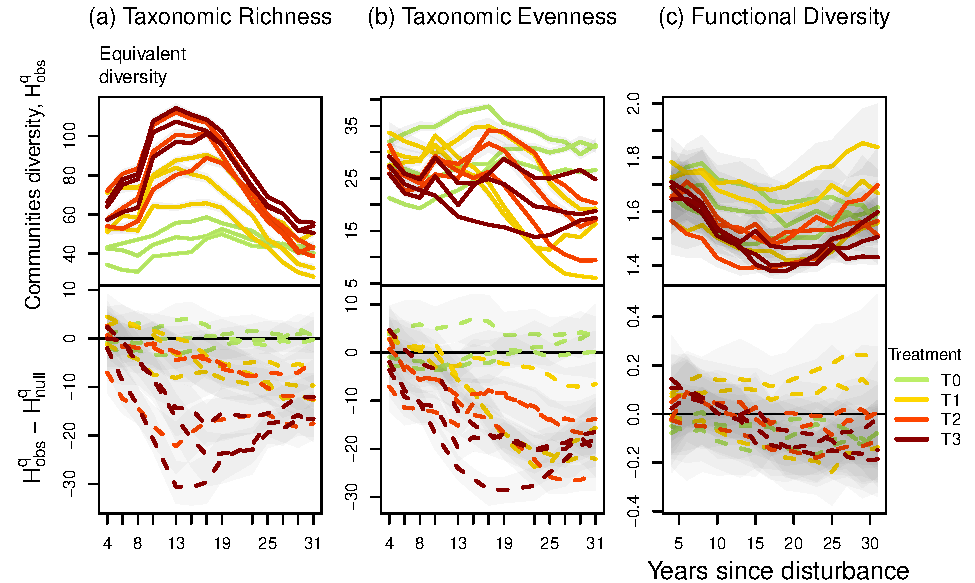
\includegraphics[width=0.8\linewidth]{RecruitmentTrajectories_files/figure-latex/DivTraj-1} 

}

\caption{Trajectories over 30 years of Richness, Shannon and Simpson diversities of punctual  recruitment (2-years laps, upper panels) and divergence to null model (lower panels). Values reported correspond to plot-level 0.025 and 0.975 percentiles (grey envelopes) and median (solid or dotted lines) obtained after 50 repetitions of the taxonomic uncertainty propagation and the functional database gap-filling frameworks. Colors correspond to the disturbance intensity (green for control, blue for T1, orange for T2 and red for T3, see Table 1 for details).}\label{fig:DivTraj}
\end{figure*}

Punctual and accumulated recruitment diversities were compared to the
stochastic trajectories of a random sampling. Richness (order 0) and
evenness (order 2) of punctual recruits remained equivalent or higher
than for a random sampling in control plots while both were lower in
disturbed plots. Disturbed plots however followed humped shaped
trajectories heading towards a recovery of the initial state (Figure
\ref{fig:DivTraj}). Accumulated recruitment richness and evenness were
higher or equivalent to those of a random sampling after low disturbance
intensity (plots T1 and some plots T2) but lower after intense
disturbance (plots T3 and a plot T2, Appendix I fig. S1).

\subsubsection{Functional Diversity and
Composition}\label{functional-diversity-and-composition}

Communities functional diversity was measured with the Rao diversity and
compared to the stochastic trajectories of a random traits shuffling. In
disturbed plots (T2 and T3), the functional diversity decreased until 15
years after disturbance (Figure \ref{fig:FunTraj}) before recovering
towards initial values. While the recovery was not achieved for the most
disturbed plots, it was faster after the low disturbance intensity and
for some T1 plots exceeded the initial values. For both disturbed and
undisturbed plots, the observed functional diversity was lower than this
of the random model, to the exception of two plots T1.

\begin{figure}

{\centering 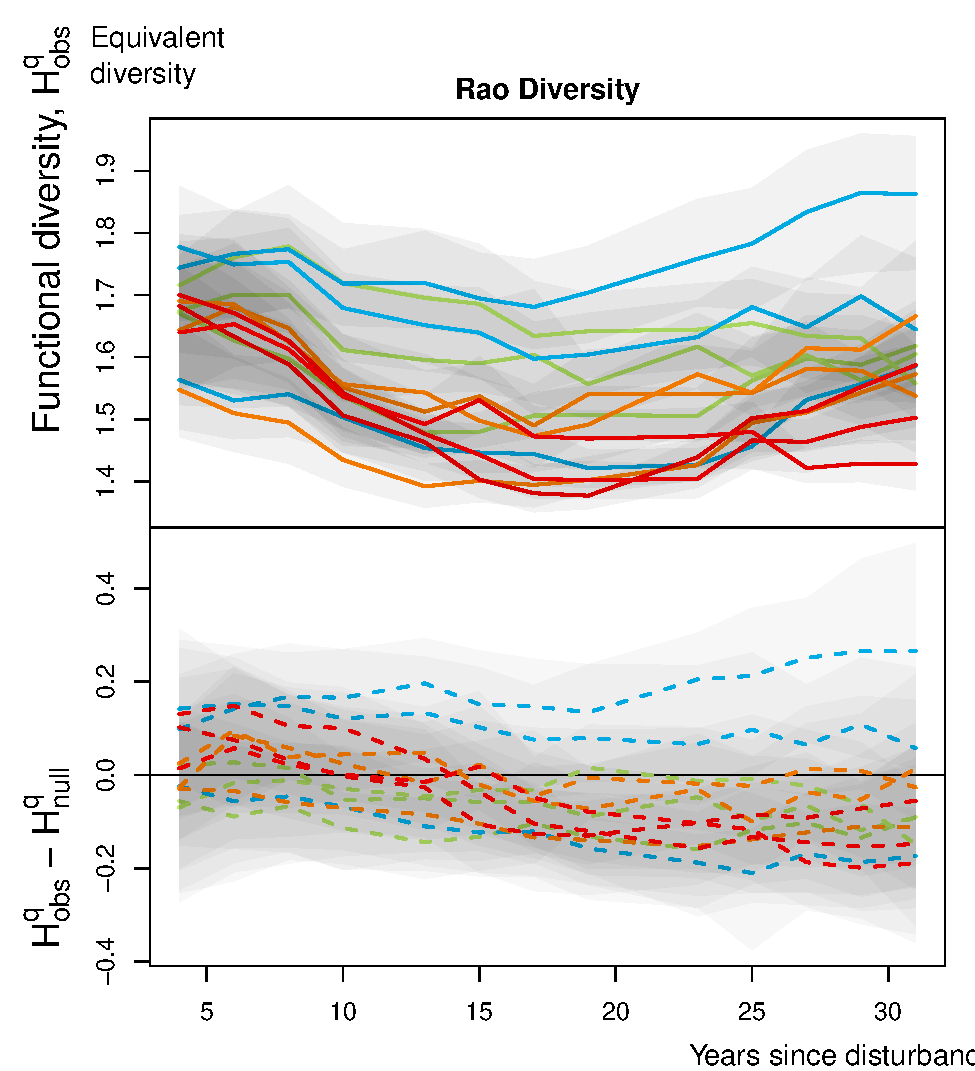
\includegraphics{RecruitmentTrajectories_files/figure-latex/FunTraj-1} 

}

\caption{Functional diversity of punctual recruited trees (2-years laps) from the 7 functional traits (upper panel) and divergence to null model (lower panel). Values reported correspond to plot-level 0.025 and 0.975 percentiles (grey envelopes) and median (solid lines) obtained after 50 run of the null model and 50 repetitions of the taxonomic uncertainty propagation and the functional database gap-filling frameworks. Colors correspond to the disturbance intensity (green for control, blue for T1, orange for T2 and red for T3, see Table 1 for details).}\label{fig:FunTraj}
\end{figure}

Trajectories of the functional traits showed a switch in disturbed plots
towards species with large exchange surface area, light tissues (high
SLA, low leaf toughness and thickness and low wood specific gravity) and
with smaller maximum height (Figure \ref{fig:CWM}). Functional traits
either followed humped shaped trajectories with an ongoing recovery or
an achieved return to the initial state (for SLA, Bark thickness and
leaf thickness and Hmax to a certain extent).

\begin{figure*}

{\centering 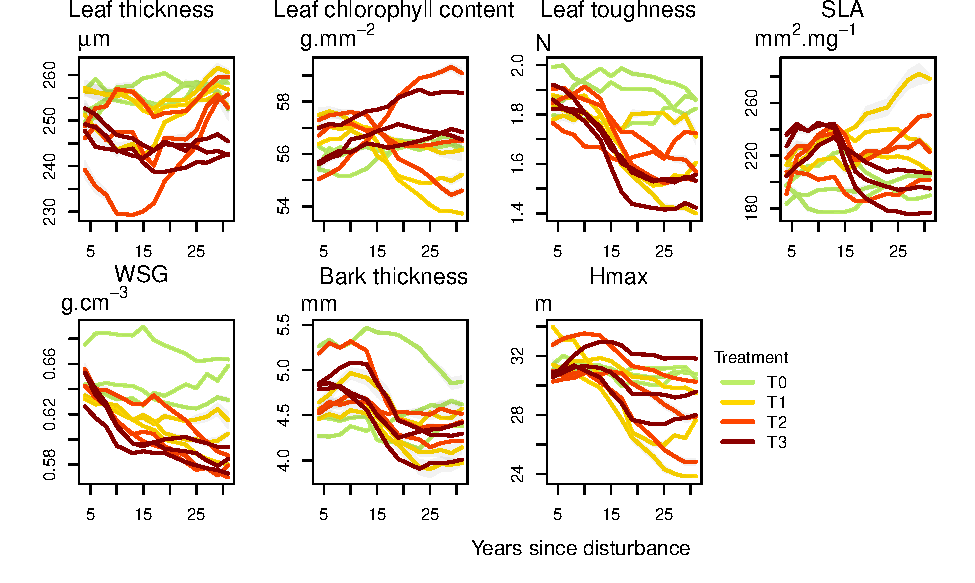
\includegraphics[width=0.8\linewidth]{RecruitmentTrajectories_files/figure-latex/CWM-1} 

}

\caption{Community weighted means (CWM) of the four leaf traits, the two stem traits and the specific maximum height. Values reported correspond to plot-level 0.025 and 0.975 percentiles (grey envelopes) and median (solid lines) obtained after 50 repetitions of the taxonomic uncertainty propagation and the functional database gap-filling frameworks. Colors correspond to the disturbance intensity (green for control, blue for T1, orange for T2 and red for T3, see Table 1 for details).}\label{fig:CWM}
\end{figure*}

\subsection{Recruitment Turnover}\label{recruitment-turnover}

In control plots species turnover remained highly stable for the 30
sampled years (Figure \ref{fig:Turnover}), reflecting a strong
similarity between the initial plots composition and the punctual
recruits. In disturbed plots, the taxonomic turnover followed a marked
humped shaped trajectory, with a maximum reached around 15 years after
disturbance and a value positively correlated to the disturbance
intensity (\(\rho_{spearman}=0.93\)). Thirty years after disturbance the
turnover of all disturbed plots had returned to low values close to
zero.

\begin{figure}

{\centering 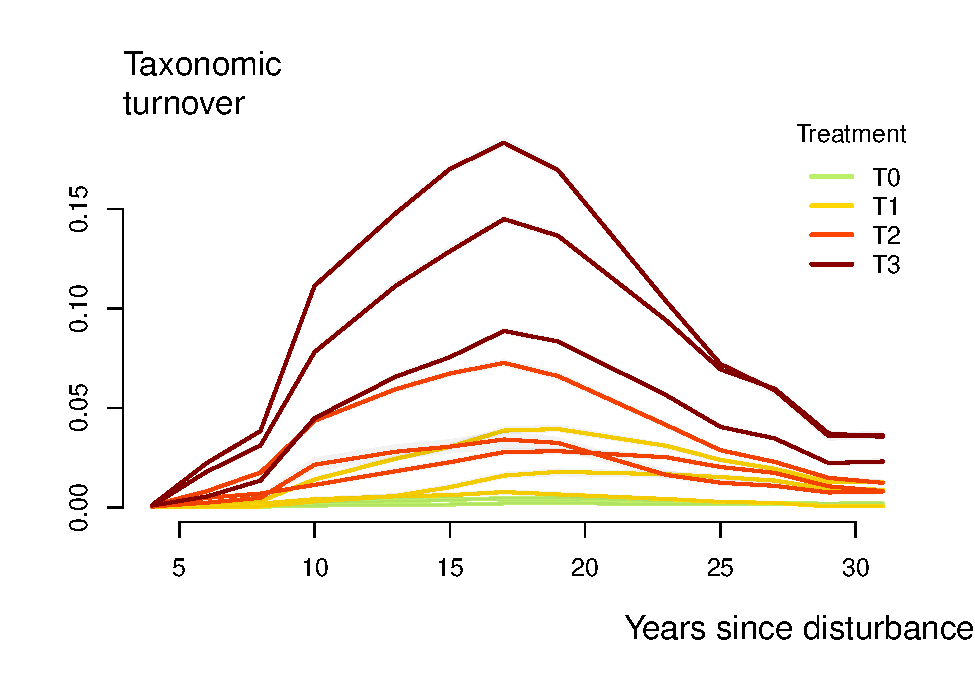
\includegraphics{RecruitmentTrajectories_files/figure-latex/Turnover-1} 

}

\caption{Trajectories over 30 years of the abundance-based turnover between recruited trees (2-years laps) and initial communities before disturbance. Values reported correspond to plot-level 0.025 and 0.975 percentiles (grey envelopes) and median (solid lines) obtained after 50 repetitions of the taxonomic uncertainty propagation framework. Colors correspond to the disturbance intensity (green for control, blue for T1, orange for T2 and red for T3, see Table 1 for details).}\label{fig:Turnover}
\end{figure}

\section{Discussion}\label{discussion}

\subsection{Three-phased trajectories from deterministic to stochatic
neutral
recruitment}\label{three-phased-trajectories-from-deterministic-to-stochatic-neutral-recruitment}

Along the 30 years, the recruitment richness and species turnover
compared to the initial composition, and the trajectories of key
functional traits (SLA and bark thickness) exhibited clear humped shaped
trajectories, revealing three distinct recruitment phases. Communities
trajectories involved a combination between the stochastic recruitment
of neutral species and the deterministic recruitment based on
competitive exclusion for resources, and a recovery of initial
stochastic and neutral recruitment.

As a first phase (0-8 years), recruited trees showed low turnover
compared to the initial composition and matched the functional diversity
of a stochastic recruitment process. This first recruitment phase,
mirroring the old-growth pre-disturbance communities, likely involved
already grown saplings (DBH \textless{} 10cm) immediately benefitting
from the increased enlightment and the alleviated competition induced by
disturbance \citep{Herault2010}.

A second phase (8-15 years) then fell into place, corresponding to
marked changes in several functional traits trajectories and to a
decrease in recruitment evenness and functional diversity. This second
phase likely incorporated true recruits, \emph{i.e.} trees germinated
from the seed bank that constitute the main part of the recruitment
\citep{Lawton1988}. The pool of species recruited then was restricted,
following deterministic processes based on species resource acquisition
strategy, and balanced the stochastic and neutral recruitment observed
in the first place \citep{Chave2004}. Indeed, sharp changes in the SLA,
wood density and leaf thickness trajectories occured after intense
disturbance and revealed the prominent recruitment of short-lived, fast
growing hard pionneer species with competitive and efficient light
acquisition \citep{Wright2004, Chave2009b, Herault2011, Reich2014}.\\
The recruitment was shaped by exclusive competition among species based
on their differences in competitive ability for light acquisition
\citep{Mayfield2010}, as already demonstrated in temperate forests
\citep{Kunstler2012}. The balance between deterministic and stochastic
processes shaping the second phase was determined by the initial
disturbance intensity. After light disturbance (T1 plots), despite a
restricted pool of recruited species, the species turnover compared to
initial state remained low. Recruited trees still mirrored the
pre-disturbance communities but recruited species were more pioneers and
light demanders, with strategies of efficient resource acquisition (high
SLA and leaf chlorophyll content) and inexpensive, short-lived tissues
(low leaf thickness and thoughness, small Hmax and low wood density and
bark thickness)
\citep{Hubbell1999, Schnitzer2001, Sheil2003, Bongers2009}. At these low
disturbance intensity the recruitment evenness and functional diversity
remained high so despite the selection of more light-demanding species
the recruitment was not overwhelmed by hard pioneers. This might be
explained by the recruitment and dispersal limitations due to the short
dispersal distances observed for tropical trees, specifically in Paracou
\citep{Leclerc2015, Scotti2015a}. After intense disturbance in contrast
(T2 and T3 plots), the recruitment rapidly differed from the
pre-disturbance composition and corresponded to a sharp increase of the
SLA and bark thickness. These drastic trajectories changes reflected an
overhelming recruitment of hard pioneers likely entailing significant
changes in communities functioning \citep{Diaz2005}.

A third recruitment phase entailed a return towards initial taxonomic
and functional diversities: although the recruited species remained
mainly light-demanding and submitted to competitive exclusion, they
displayed increasing functional diversity and similarity with the
initial composition. Initial stochastic recruitment eventually
recovered, restoring the equilibrium between neutral and deterministic
processes \citep{Lawton1988, Chave2004, Mayfield2010}.

Recruitment trajectories of disturbed and undisturbed areas were
identical, supporting a recruitment success and an enlightement
homogeneous in undisturbed communities \citep{Dalling2002} and evenly
increasing in disturbed communities through large gaps edge effects
\citep{Ruger2009}.

\subsection{The questioned completeness of communities
resilience}\label{the-questioned-completeness-of-communities-resilience}

After 30 years, although taxonomic and functional diversity had
recovered initial values the recruitment processes remained constrained
by the deterministic selection of recruited species, contrasting with
the stochastic recruitment of undisturbed forests. The stochastic
recruitment proved eventually resilient and ensured communities
taxonomic convergence towards different stable equilibria, but lasted
for several decades.

The recovery of both recruitment processes and initial composition and
diversity meant the maintenance of the taxonomic differences between
communities. Multiple stable equilibria, corresponding to the initial
commmunities restored after disturbance, were maintained as predicted
for highly diverse and productive ecosystems \citep{Chase2003}. These
different equilibria besides oriented communities trajectories towards
their initial composition, as suggested with the involvement of
pre-disturbance grown saplings and local seed bank and as already
observed consistently with other case study
\citep{Dalling2002, Anderson2007}.

In contrast, recruitment functional diversity and some traits
trajectories were similar among treatments and recovered quickly,
translating communities convergence in the functional space and their
fast functioning recovery despite their divergence in the taxonomic
space \citep{Fukami2005}. This confirmed previous results from the
Paracou experiment, conducted 10 years \citep{Molino2001} and 20 years
\citep{Baraloto2012a} after disturbance, where the early signs of the
resilience of taxonomic and functional composition had been detected.

Communities recovery was then consistent but slow, specifically for
taxonomic diversity and several functional traits that remained altered
30 years after disturbance. Besides, the recovery invovled and probably
altered the seed bank stock, hence changing the diversity of the
recruitable species and the resilience of the communities
\citep{Norden2009}.

\section{Conclusion}\label{conclusion}

The hindsight of the 30 years of forest monitoring highlighted a
three-phased disturbance response, defined by the balance between
stochastic neutral processes and determinisitic recruitment based on
species strategy of light acquisition. Communities trajectories were
first driven by the stochastic recruitment of already-grown saplings
mirroring pre-disturbance communities before it was shaped by true
recruits from the seed bank slected through the competitive exclusion
for light. After intense disturbance the second recruitment phase was
dominated by short-lived hard pioneers that drastically changed
communities diversity and functioning. A third phase eventually carried
out the recovery towards the initial communities with the recovery of
stochastic recruitment progressively balancing competitive exclusion.
Recruitment trajectories demonstrated a fast functional recovery driving
communities convergence in the functional space, and a decades long
taxonomic recovery that maintained the initial composition differences.
Even though the accurate impact on the seed bank remains to be
clarified, communities recovery was tangible but slow and entailed great
caution regarding forests management guidelines aiming to a complete
recovery of ecosystems.

\begin{center}\rule{0.5\linewidth}{\linethickness}\end{center}

%----------------------------------------------------------------------------------------
%	REFERENCE LIST
%----------------------------------------------------------------------------------------

\bibliographystyle{mee}
\makeatletter
% The filename has .bib extension the must be eliminated
\filename@parse{references.bib}
% parse stores the file name in base. Extension starts at the first dot, so don't use dots in file names.
\bibliography{\filename@base}
\makeatother


%----------------------------------------------------------------------------------------

\end{document}
